\documentclass[10pt]{article}
\usepackage[margin=0.65in]{geometry}
\usepackage[T1]{fontenc}
\usepackage{lmodern,graphicx,booktabs,hyperref}
\setlength{\parindent}{0pt}\setlength{\parskip}{6pt}
\setlength{\emergencystretch}{3em}
\begin{document}
{\Large\bfseries CPU numerator comparison: 360 completed calls}

23 November 2026. Unsigned local records \texttt{PCC-20261123-70a35c}
(native observations) and \texttt{PCC-20261123-169bed} (metadata checks).
Authenticated execution standing is not established. [pcc:unverified]

\textbf{Recorded outcome.} All 360 calls complete on 12 fixed public targets:
36 warmups and 324 measured observations, nine processes per arm/target.
Full certificate bytes and structural counters agree per target across every
arm/repeat. All 360 external Native replays, 360 OpenSSL positives and 720
required corruption controls pass. Supervisor/all three phases exit zero, no
physical stop; all 295 post-call input hashes match. [pcc:unverified]

\textbf{Protocol/export gate.} The original protocol-bound canonical check
\textbf{fails with 324 seed-table findings}. Its \texttt{explicit\_list}
convention derives numeric instance IDs, replicates 0--8 and cycled seeds;
the frozen native contract uses case--seed IDs, rounds 1--9 and a fixed seed
per target. Original protocol/export/raw data remain unchanged. A separate
schema/flow/file-only check has zero findings and does not accept that
protocol/export pairing. The future-only corrected draft is unadopted and
cannot backdate prospective standing. See \path{EXPORT-ERRATA.md}.
[pcc:unverified]

\textbf{Actual comparator.} a/c are the same staged-numerator parent; b is the
current reverse-pass numerator candidate. Two common 108-input source snapshots
differ only in that library file. Same six 20/24/28/32/36/40-bit field fixtures,
order bits 20/25/28/32/36/41, public target seeds 101/202, m8/batch64 and fixed
caps. Targets come from public x-search; no target scalar is supplied. Warmups,
historical runs and synthetic controls are excluded from measured data.
[pcc:unverified]

\textbf{Observed timing comparison.} On the largest two targets, a-to-b complete
medians are 15.889932035 to 14.912780968 seconds and 13.419740394 to
12.781461206 seconds; c medians are 15.406181760 and 13.185250292 seconds.
Smaller targets are mixed. The c/40-bit/seed202 maximum of 46.241018449 seconds
is retained. All targets, A/A observations and full ranges appear below.
Shared-host L0 clocks, known source labels, build paths and ASLR limit
interpretation. No significance/equivalence decision or exponent fit is made.
CPU time, per-process peak RSS and complete counted S remain unmeasured.
[pcc:unverified]

\textbf{Clock boundaries.} Internal complete includes curve/target construction,
all setup/trials, oracle, reduction, internal replay, additional Archive
verification and serialization. It excludes launch, corruption control, I/O,
external Native replay and OpenSSL audit. Driver encloses worker process plus
external Native replay; oracle is an included subphase. All three full-range
summaries remain in the unchanged primary CSV. [pcc:unverified]

\textbf{Execution and custody.} Published frozen packet 51ac3d74, protocol
5bcd3100 frozen 14:30:46 UTC; main starts 14:44:47, driver ends 15:03:27,
audit/supervisor ends 15:03:34. One attempt, zero retry/resume, balanced measured
positions, no concurrent builds/tests. Sampled whole-cgroup peak
14,327,767,040 bytes includes retained research; it is not process RSS.
Worker-only 4 GiB virtual limit and 1500/120/120-second phase ceilings are
unchanged. All 302 pre-run checkpoint payload hashes were read back, including
all 295 main inputs. Reviews 10--14 stay immutable. [pcc:unverified]

\textbf{Reproduction record.} Source-prehashed post-run Rust adapter passes six
controls and strict Clippy; initial lint failure is retained. It executes no
solver/replay/primary analysis. All CSV numeric tokens and status JSON values
are preserved. The 2,936,344-byte export and full certificates/status/events
stay local, with exact receipts; S3 is excluded. Compact original worker CSV,
schedule, summary, control progress and phase receipts accompany this report.
Remote full replay and signed execution standing remain open. [pcc:unverified]

\small Sources: \path{MAIN-OUTCOME.md}, \path{EXPORT-ERRATA.md},
\path{records/main/}, \path{checks/main-result/}.\par
Full payload: \path{/tmp/ecdlp-cpu-comparison-20261123/}.\par
\url{https://github.com/isogeny-labs/crypto/pull/4996}

\clearpage
{\Large\bfseries Frozen native summary: all 36 target/arm groups}

The original primary SVG, with complete-time medians and full observed ranges.
Each group has nine measured processes. All 36 warmups are excluded.
Linear scale preserves the native output; the table on the next page gives
small values numerically. [pcc:unverified]

\begin{center}
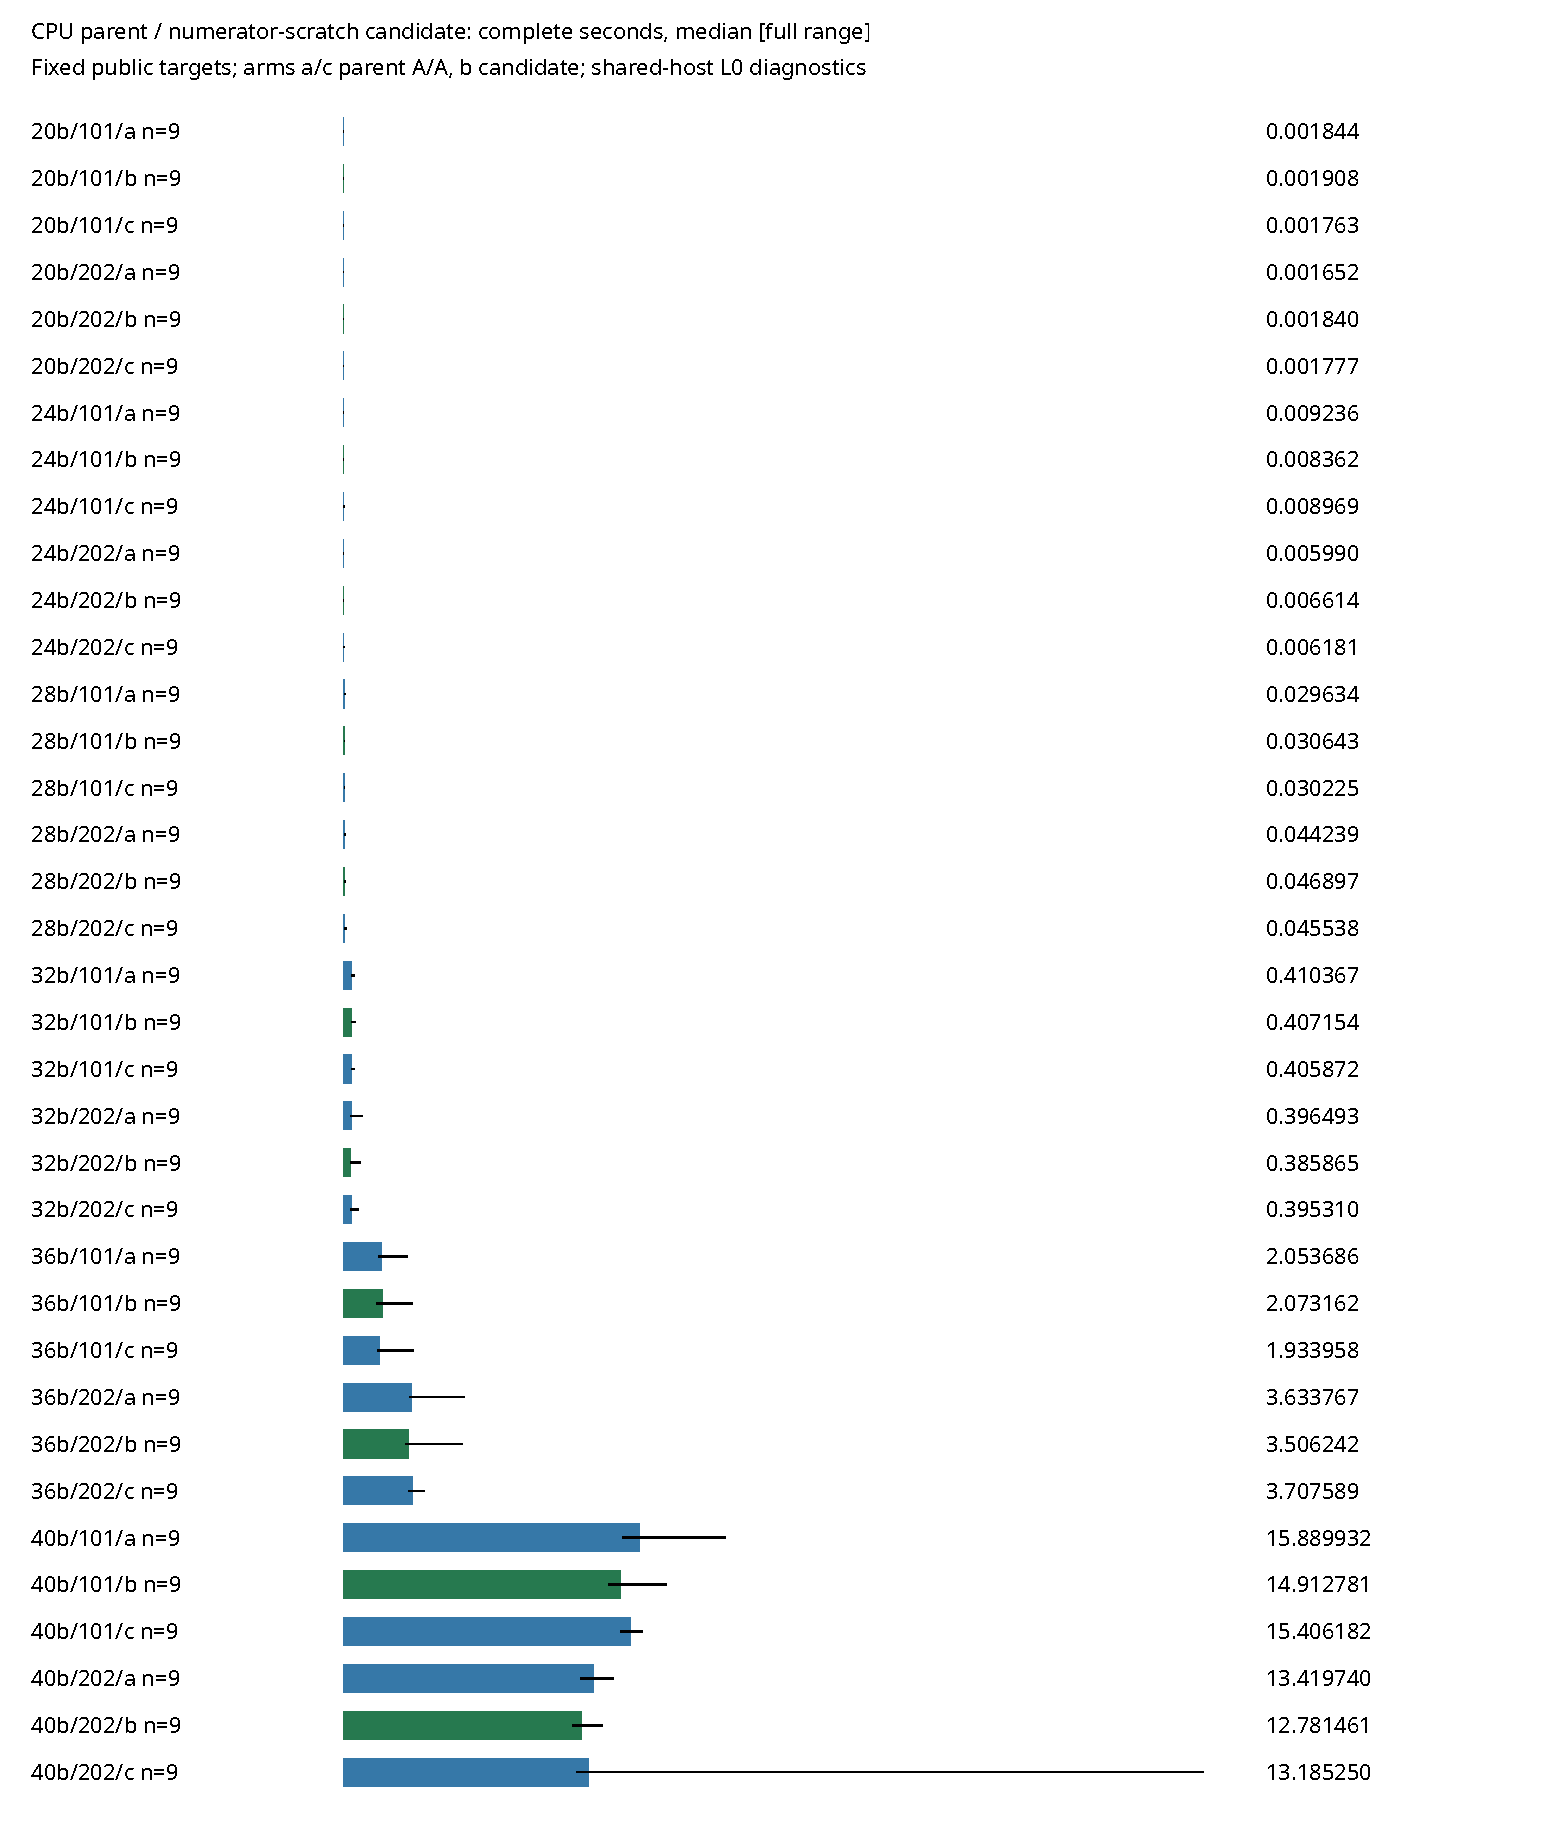
\includegraphics[width=\linewidth,height=8.0in,keepaspectratio]{latency.pdf}
\end{center}
\small Source: original \path{main/latency.svg}; original bytes are copied to
\path{records/main/latency.svg}. Rendering adds no observations or inference.

\clearpage
{\Large\bfseries Complete-clock medians and full ranges}

a/c: same parent; b: reverse-pass candidate. Ratios use the named parent's
median divided by this row's median; values above one mean this row has the
lower recorded median. A/A can be read in a/c rows. Times round to six decimal
places, ratios to three; full precision stays in the primary CSV.
[pcc:unverified]

\begin{center}\small
\setlength{\tabcolsep}{5pt}
\begin{tabular}{rrrrrrrrr}\toprule
Bits & Seed & Arm & $n$ & Min (s) & Median (s) & Max (s) & $a$/arm & $c$/arm \\ \midrule
20 & 101 & a & 9 & 0.001595 & 0.001844 & 0.004427 & 1.000 & 0.956 \\
20 & 101 & b & 9 & 0.001628 & 0.001908 & 0.002607 & 0.966 & 0.924 \\
20 & 101 & c & 9 & 0.001555 & 0.001763 & 0.003427 & 1.046 & 1.000 \\
20 & 202 & a & 9 & 0.001535 & 0.001652 & 0.002516 & 1.000 & 1.076 \\
20 & 202 & b & 9 & 0.001552 & 0.001840 & 0.002358 & 0.898 & 0.966 \\
20 & 202 & c & 9 & 0.001562 & 0.001777 & 0.002957 & 0.930 & 1.000 \\
24 & 101 & a & 9 & 0.007670 & 0.009236 & 0.013289 & 1.000 & 0.971 \\
24 & 101 & b & 9 & 0.007820 & 0.008362 & 0.013171 & 1.105 & 1.073 \\
24 & 101 & c & 9 & 0.007863 & 0.008969 & 0.025208 & 1.030 & 1.000 \\
24 & 202 & a & 9 & 0.005317 & 0.005990 & 0.006483 & 1.000 & 1.032 \\
24 & 202 & b & 9 & 0.005584 & 0.006614 & 0.008663 & 0.906 & 0.935 \\
24 & 202 & c & 9 & 0.005687 & 0.006181 & 0.014601 & 0.969 & 1.000 \\
28 & 101 & a & 9 & 0.027787 & 0.029634 & 0.100965 & 1.000 & 1.020 \\
28 & 101 & b & 9 & 0.027603 & 0.030643 & 0.058088 & 0.967 & 0.986 \\
28 & 101 & c & 9 & 0.027760 & 0.030225 & 0.064898 & 0.980 & 1.000 \\
28 & 202 & a & 9 & 0.041774 & 0.044239 & 0.069214 & 1.000 & 1.029 \\
28 & 202 & b & 9 & 0.040692 & 0.046897 & 0.068624 & 0.943 & 0.971 \\
28 & 202 & c & 9 & 0.042527 & 0.045538 & 0.137959 & 0.971 & 1.000 \\
32 & 101 & a & 9 & 0.393426 & 0.410367 & 0.604814 & 1.000 & 0.989 \\
32 & 101 & b & 9 & 0.392260 & 0.407154 & 0.626229 & 1.008 & 0.997 \\
32 & 101 & c & 9 & 0.397838 & 0.405872 & 0.561893 & 1.011 & 1.000 \\
32 & 202 & a & 9 & 0.374288 & 0.396493 & 1.027277 & 1.000 & 0.997 \\
32 & 202 & b & 9 & 0.370445 & 0.385865 & 0.923240 & 1.028 & 1.024 \\
32 & 202 & c & 9 & 0.374905 & 0.395310 & 0.769431 & 1.003 & 1.000 \\
36 & 101 & a & 9 & 1.867032 & 2.053686 & 3.442045 & 1.000 & 0.942 \\
36 & 101 & b & 9 & 1.757571 & 2.073162 & 3.675162 & 0.991 & 0.933 \\
36 & 101 & c & 9 & 1.834992 & 1.933958 & 3.758694 & 1.062 & 1.000 \\
36 & 202 & a & 9 & 3.551258 & 3.633767 & 6.493595 & 1.000 & 1.020 \\
36 & 202 & b & 9 & 3.323049 & 3.506242 & 6.402174 & 1.036 & 1.057 \\
36 & 202 & c & 9 & 3.480727 & 3.707589 & 4.366019 & 0.980 & 1.000 \\
40 & 101 & a & 9 & 15.016292 & 15.889932 & 20.538337 & 1.000 & 0.970 \\
40 & 101 & b & 9 & 14.230732 & 14.912781 & 17.384026 & 1.066 & 1.033 \\
40 & 101 & c & 9 & 14.913066 & 15.406182 & 16.092032 & 1.031 & 1.000 \\
40 & 202 & a & 9 & 12.765976 & 13.419740 & 14.505816 & 1.000 & 0.983 \\
40 & 202 & b & 9 & 12.316120 & 12.781461 & 13.912869 & 1.050 & 1.032 \\
40 & 202 & c & 9 & 12.521786 & 13.185250 & 46.241018 & 1.018 & 1.000 \\
\bottomrule\end{tabular}

\end{center}

\small Source: native frozen \path{main/summary.csv}; the post-run qualified
adapter formats these existing values without recomputing statistics.
Full driver/oracle ranges remain in that CSV. [pcc:unverified]

\textbf{Continuing work.} Keep the complete parent/candidate/A-A reference and
correct future protocol identity/seed semantics before new data. Extend complete
counted accounting and independent target coverage, while continuing the
source/history/cost proof bridge from the existing precision audit. The
classical research goal remains active.

\textbf{Bounded prior-art read.} The local autoresearcher snapshot supplies
EXP-HZM-001 and the corrected July18 zero-minor triage; their explicit
enumeration/model conclusions retain their scope. The primary collinearity
paper uses real-polynomial sign tests; no prime-field implementation follows
from that model alone. This read prevents treating an archived enumerative
reformulation as untried; it is not a novelty clearance. [pcc:unverified]

\url{https://arxiv.org/html/2607.09814v2}\par
\url{https://arxiv.org/html/2003.09533v3}\par
\path{checks/main-result/lead-scout-read-receipt.json}
\end{document}
